\section{Experimental Methods}
\label{sec:experiment}
The task that trial subjects were faced with was designed to facilitate
comparison between the subjects' decisions and those that would be made by a
particle filter. Modeling sequential, online category learning was useful both
because that was the type of categorization algorithm developed in previous
work, and because it has a straightforward manifestation in a constrained human
task. Trial subjects were presented with stimuli images, sequentially, and asked
to assign each image into a group. Once the image was placed in a group, the
subject was not allowed to switch the image to another group. The instructions
given to each subject can be viewed in the Appendix, Figure
\ref{fig:instructions}.

The stimuli used were 100 by 100 pixel images. A sample
stimulus can be viewed in Figure \ref{fig:stimulus}. Each pixel in an
image is a shade of gray between white and black, with 256 possible grayscale
values. This type of stimuli is convenient because it is directly interpretable
for the inference algorithm: each pixel-block is a feature, and each feature can
take one of 256 possible values. This type of stimuli was also considered
attractive because of the difficulty for the human subject of categorizing the
images. It was thought that this difficulty would compel the subjects to rely on
subconscious processes for categorization. In retrospect, as is addressed in
Section \ref{sec:discussion}, the high dimensionality of the images may have
made it too difficult for the brain to categorize the images effectively, and
may have lessened the interpretive power of the results. Figure
\ref{fig:clusterer} shows how the interface would appear for a mostly completed trial.

\begin{figure}
\centering

\includegraphics[scale=1]{img/stimulus.png}
\caption{A sample stimulus to be categorized. The stimuli were generated from
  10 by 10 matrices of values between 0 and 255, where the value determined the
  grayscale value. The images were smoothed.}
\label{fig:stimulus}
\end{figure}

Workers from Mechanical Turk were hired to be trial subjects. They were presented
with a website on which to conduct the trial: each worker was first shown the
instruction page in Figure \ref{fig:instructions}, and then were brought to the
page on which the trial was conducted, show in Figure \ref{fig:clusterer}  All
the actions performed by the subject were collected in a database to be used for
later analysis.

\begin{figure}
\centering
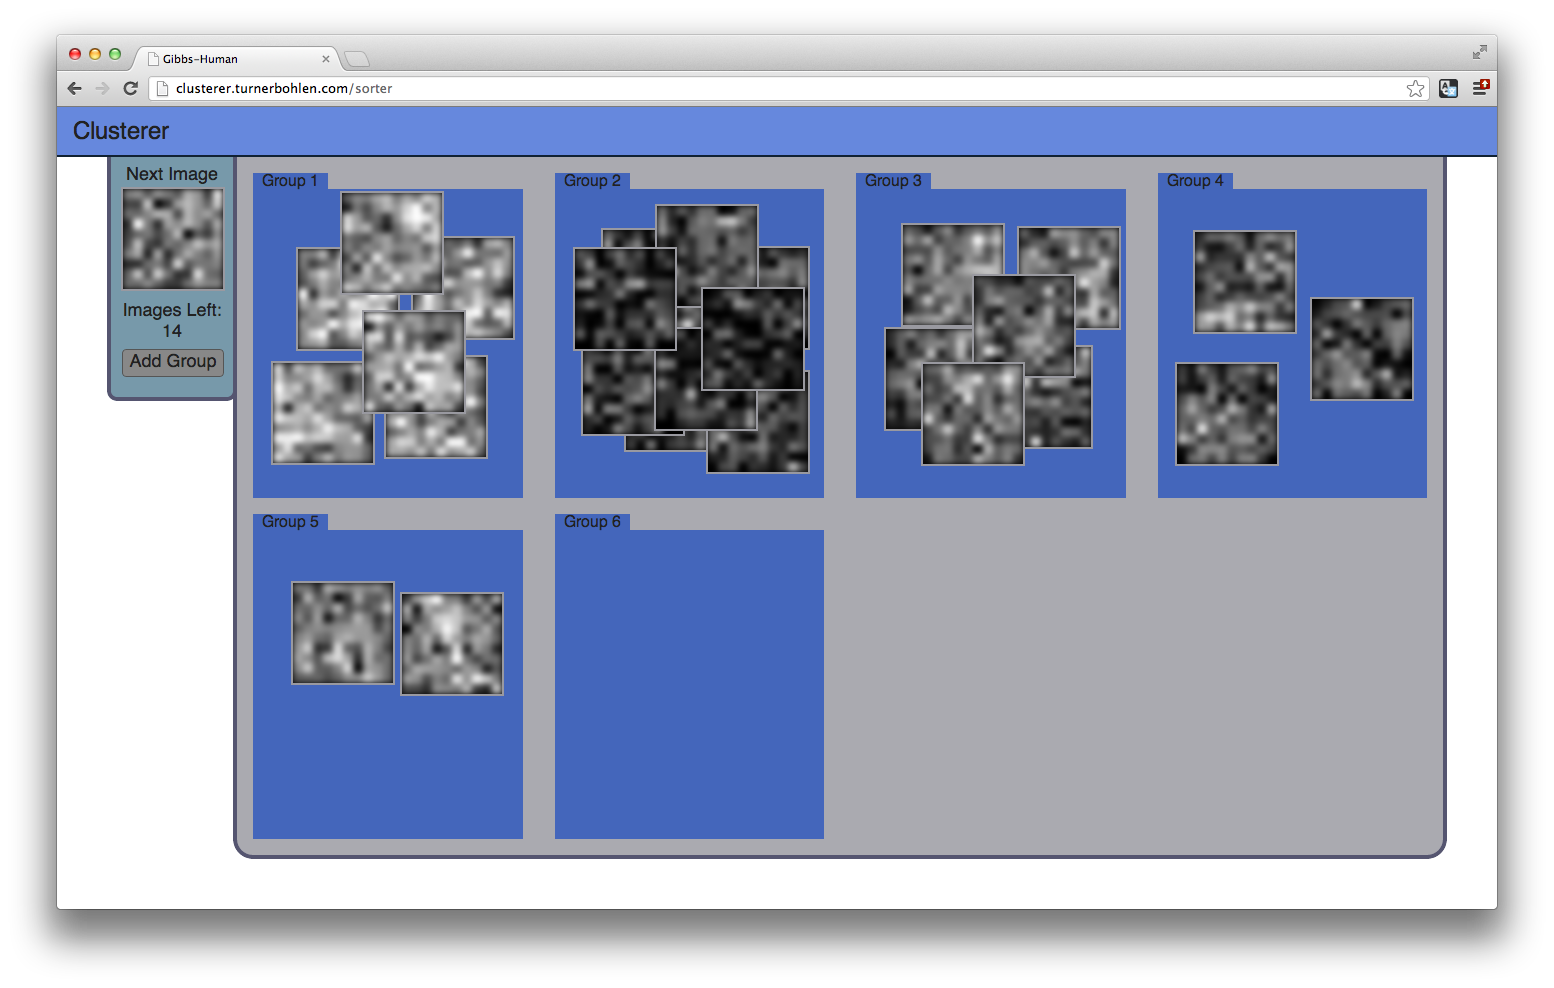
\includegraphics[width=5.6in]{img/clusterer.png}
\caption{Interface through which a trial was completed. Images are dragged from
  the 'Next Image' box into one of the groups. Once an image was placed in a
  group, it could not be switched into another group.  The subject was limited
  to creating 8 groups.}
\label{fig:clusterer}
\end{figure}
